\chapter{Stored Loss and Monetized Rescue: $S_t$ and $P_1/P_0$}
\label{ch:storedloss}

\textit{Bridge.} Chapter 5 priced gates ($\psi$) and caps ($K$) at the claim level and showed the waterfall at $1.00$ median secured vs $0.213$ median general unsecured. This chapter prices delay at the system level. Unpaid remainders do not vanish when $\phi<1$. They accumulate as a stock $S_t$ that accounting can leave at par until the wall forces recognition, then get socialized through the price level as $P_1/P_0$. Chapter 7 will show what happens when the apex itself has $A=0\Rightarrow K=0$ and treaty gates drive $g_4\to0$ so even the wall has no enforcer -- bounded by the South Africa precedential-chill null \texttt{PMC8422681} and the Gilens--Bashir debate on how large $g_4\to0$ is for citizens. Picture a basement where the pump log reads dry for eleven quarters while water rises behind the wallboards. The log is the income statement. The water is the stock. The wall is not a new storm. It is the water arriving all at once.

\textit{Grade for this chapter: measured on BIS credit-gap inversion ($+11.6\to-9.4$), on charge-off and provisioning flows ($0.98\to3.02\%$, $5.7\times$), on FDIC aggregates with IMF cross-match ($112\to430\%$ coverage on $4.9599\%$ cross-matched NPL), on World Bank and IMF NPL panels across jurisdictions (to $45.97\%$), on BIS DSR flow masking ($18.5\to14.1$), and on CPI/M2 levels and S\&P defaulted-debt stocks ($\$627.7$B). The $S_t$ law is formal; the direction and bearer of $S_t$ are measured where series agree. DSR interpretation is flow-vs-stock, flagged as such.}

\section{Two numbers, one sentence each, and the law that links them}
\label{sec:stored-defs}

We reuse $\psi$, $K$, $\phi$ from Chapter 5 (\ref{eq:psi5}--\ref{eq:phi5}) and add the two stock-and-flow numbers for this chapter, each with a line of worked arithmetic so a new reader can check the ledger without trusting prose.

$S_t$ is stored loss, the off-book stock:
\begin{equation}
S_t = S_{t-1}+E_t-R_t-Q_t,
\label{eq:St6}
\end{equation}
where $E_t$ is new extraction or loss creation in period $t$, $R_t$ is realized recovery, and $Q_t$ is write-offs or forgiveness. \textit{One line:} new holes minus what you clawed back minus what you admitted will never come back, compounding when you keep $R_t$ and $Q_t$ low. Worked: start $S_0=0$, each period $E=10$, $R=2$, $Q=1\Rightarrow\Delta S=10-2-1=7$, so $S_{10}=70$ after ten periods. Reports showed $3$ of recovery plus write-off against $10$ of extraction -- modestly negative income -- while the stock quietly became $70$ off or under-provisioned. When rolls fail, $Q$ must spike. That spike is the wall; it was not a new shock but the stock coming due.

$P_1/P_0$ is dilution, the price level after $G$ of outside money is created against claims base $L$:
\begin{equation}
P_1/P_0 = L/(L-G),\qquad 0\le G<L,
\label{eq:P6}
\end{equation}
with $P_0$ before, $P_1$ after. \textit{One line:} if you cover stored loss with new money instead of assigning it to a junior class, every old claim buys $P_0/P_1$ of what it did. Worked: $L=100$, $G=20\Rightarrow P_1/P_0=100/80=1.25$, so prices rise $\approx25\%$ and each old claim buys $0.80$, a $20$-point haircut without a legal default. Measured footprint version: CPI $1.0391$ on M2 $1.1741$ ($2008\to2010$) and CPI $1.1532$ on M2 $1.3804$ ($2020\to2022$) \texttt{finance\_falsify\_v1.json}; at $P_1/P_0=1.1532$, a nominal claim buys $1/1.1532\approx0.867$, a $13.3$-point haircut via prices.

The law is accounting, not theory. If $E_t>R_t+Q_t$ for many periods, $S_t$ climbs even while income looks calm \textit{(formal)}. If $R_t$ is low because $K$ binds and $Q_t$ is low because you extend or evergreen, the climb is silent \textit{(mechanism)}. The wall is $S_t$ coming due at once because rolls are discrete. Rescue is the choice to let $G$ absorb $S_t$ and push loss into $P_1/P_0$ instead of into a named $\phi$ cut. Who bears it moves; the amount does not. The system view is therefore: Ch.~5's $\psi$ and $K$ decided who \textit{would} have absorbed it in the waterfall; $S_t$ decides how much must be absorbed; $P_1/P_0$ decides who absorbs it when absorption is socialized. Two stories compete for every rescue and both hide half. The salvation story says the bailout erased the loss. But conservation holds: the amount never moves, only the bearer. The blame story says someone stole it in the night. But no theft was needed; par accounting plus new money moved it through prices without touching a vault. What remains standing: every rescue is a choice of bearer, never a reduction of loss.

\section{At par is a choice: how accounting stores $S_t$ without moving price}
\label{sec:par}

US bank books carry most loans and many securities at par or amortized cost until a trigger forces fair value. That is not a footnote quirk. It is the store. Par says a $\$100$ face that trades at $\$70$ is still $\$100$ on the balance sheet, with the $\$30$ in $S_t$, not in CET1, until a sale, a rating, or a provision forces $Q_t$. Two labels, same economics, different timing. Trading desks live in $P_1/P_0$. Loan books live in $S_t$.

The distinction matters because triggers are managed. Maturity extension pushes the sale trigger out. Forbearance pushes the $Q_t$ trigger out. Guarantee keeps the instrument performing so provisioning stays $R_t$-thin. Each move preserves par on paper while $S_t$ builds in substance. Formal capital looks adequate because $S_t$ is not yet forced through provisions -- which is why the next sections measure gap, coverage, and flows rather than quoting capital ratios. \textit{Grade: mechanism (accounting identities); measurement follows.}

\section{The gap that predicted the wall: $+11.6\to -9.4$}
\label{sec:bis-gap}

\textit{Grade: measured (BIS WS\_CREDIT\_GAP bulk, $6.2$M records, on disk, \texttt{finance\_falsify\_v1.json}).}

The BIS credit-to-GDP gap for the US, the deviation of private credit from its long-run trend, moves ahead of charge-offs by design. It is the macro proxy for $S_t$ accumulation.

\[
\begin{array}{lccccc}
\text{Quarter} & 2006\text{Q4} & 2007\text{Q4} & 2008\text{Q4} & 2009\text{Q4} & 2010\text{Q4} \\
\text{Gap (\% pts)} & 10.11 & 11.63 & 6.68 & 1.24 & -9.43 \\
\end{array}
\]

\texttt{finance\_falsify\_v1.json} records $10.1071$, $11.6341$, $6.681$, $1.2405$, $-9.4288$ from $2006$Q4 to $2010$Q4. Shorthand $+11.6\to-9.4$ is the swing from peak to trough, about $21$ percentage points in three years. A positive gap that large says credit is about $11$ points above trend; a negative gap that large says deleveraging is about $9$ points below it. The wall sits between them, and $S_t$ is the stock that had to be recognized or diluted to get from one to the other.

Novelty: this is not a subtle leading indicator. $+11.6$ in $2007$Q4 is an extreme print by postwar standards. The $2008$Q4-to-$2009$Q4 collapse in the gap tracks the wall quarter by quarter, which is exactly what a stored stock that is suddenly provisioned does. The sign flip is the ledger, not the economy. Arithmetic check: peak-to-trough $11.6341-(-9.4288)=21.0629$ points; $2007$Q4-to-$2009$Q4 alone $11.6341-1.2405=10.3936$ points in two years.

\section{Flows that confess after the fact: charge-offs to $3.02\%$ and provisions $5.7\times$}
\label{sec:flows}

\textit{Grade: measured on FFIEC CDR aggregates (regex over instance docs), FRED CORALACBS (charge-offs), FDIC BankFind API (asset-weighted), IMF FSIC (cross-match). All held.}

Charge-offs are realized $Q_t$ in dollars per loan dollar. FRED CORALACBS \texttt{fred\_CORALACBS.csv} and \texttt{finance\_falsify\_v1.json}:

\begin{center}
\small
\begin{tabular}{lcc}
\toprule
Print & Date & Value (\%) \\
\midrule
Calm & $2008$Q1 & 0.98 \\
Peak & $2010$-$01$-$01$ & 3.02 \\
\midrule
Rise &  & $3.02/0.98\approx3.08\times$ \\
\bottomrule
\end{tabular}
\end{center}

That is a threefold rise \textit{after} the gap had already signaled the wall. $S_t$ was stored in $2007$ (gap $+11.6$), charge-offs were still $0.98$. By peak $Q_t$ is $3.02$, gap is already $-9.43$ or headed there, and the stock is being forced. Flows lag stocks. That is the point of storing.

Provisions are the flow that precedes coverage. FFIEC CDR aggregates, quarters $2009$Q4 ($7{,}321$ banks) and $2026$Q2 ($4{,}297$ banks), XBRL via \texttt{ffiec-data-collector} $2.0.0$rc2, held as \texttt{ffiec\_provisions\_wall\_v1.json}:

\begin{center}
\small
\begin{tabular}{lccc}
\toprule
Quarter & ALLL stock (\$B) & Loans (\$B) & Provision flow (\$B) \\
\midrule
$2009$Q4 & 43.7 & 6,310.0 & 233.6 \\
$2026$Q2 & 59.2 & 13,274.7 & 40.7 \\
\bottomrule
\end{tabular}
\end{center}

Provision flow at the wall is $233.6$B versus $40.7$B in the $2026$ calm, a $5.74\times$ print ($233.6/40.7\approx5.74$). ALLL stock barely moves $43.7\to59.2$ ($+35\%$) while loans double $6{,}310\to13{,}275$ ($+110\%$), so ALLL/loans sits $0.69\%$ at the wall ($43.7/6{,}310$) and $0.45\%$ in calm ($59.2/13{,}275$, CECL-era stock). The flow spikes while the stock looks thin. That is $R_t+Q_t$ racing to catch $S_t$, not $S_t$ being small. ALLL is a stock that should have been there earlier; provisions are the catch-up. \textit{Grade note:} NPL denominator needs full RC-N line mapping across MDRM vintages, deferred, so FRED charge-offs plus World Bank NPL stand in for $Q_t$ validation rather than a single FFIEC NPL coverage ratio.

\begin{figure}[h]
\centering
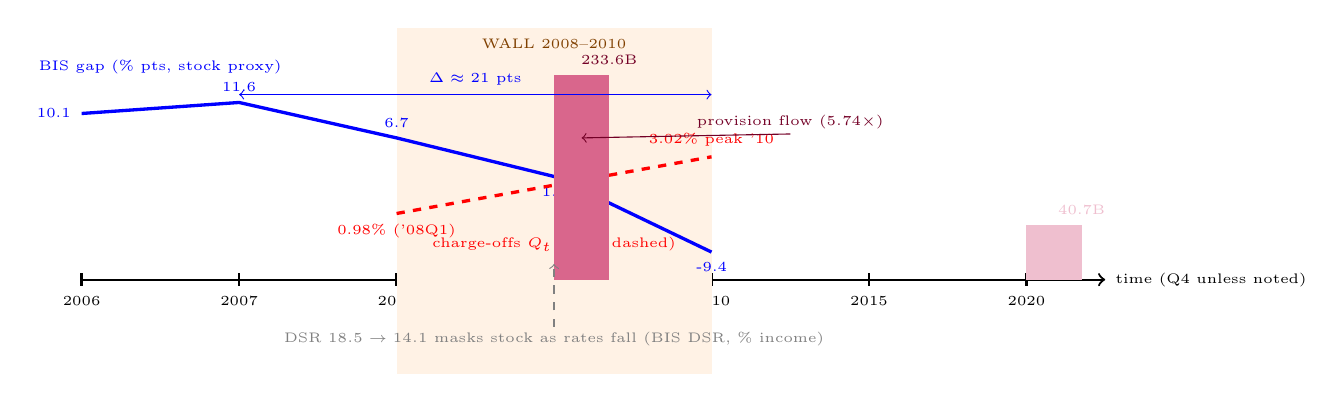
\begin{tikzpicture}[thick]
% timeline axis 2006 -> 2026
\draw[->] (0,0) -- (13,0) node[right,font=\tiny] {time (Q4 unless noted)};
\foreach \x/\yr in {0/2006,2/2007,4/2008,6/2009,8/2010,10/2015,12/2020}
  \draw (\x,0.08) -- (\x,-0.08) node[below,font=\tiny] {\yr};
% wall shading 2008-2010
\fill[orange!10] (4,-1.2) rectangle (8,3.2);
\node[font=\tiny,orange!50!black] at (6,3.0) {WALL 2008--2010};
% BIS gap line (scale: gap % pts -> y = 1.2 + gap*0.09, so 11.6 ~2.25, -9.4 ~0.35)
\draw[blue,very thick] (0,2.11) node[left,font=\tiny,blue] {10.1} -- (2,2.25) node[above,font=\tiny,blue] {11.6} -- (4,1.80) node[above,font=\tiny,blue] {6.7} -- (6,1.31) node[below,font=\tiny,blue] {1.2} -- (8,0.35) node[below,font=\tiny,blue] {-9.4};
\node[font=\tiny,blue] at (1,2.7) {BIS gap (\% pts, stock proxy)};
% charge-off line (scale: % -> y = 0.5 + %*0.35, so 0.98~0.84, 3.02~1.56)
\draw[red,very thick,dashed] (4,0.84) node[below,font=\tiny,red] {0.98\% ('08Q1)} -- (8,1.56) node[above,font=\tiny,red] {3.02\% peak '10};
\node[font=\tiny,red] at (6,0.45) {charge-offs $Q_t$ (flow, dashed)};
% provision flow bars (scale: $B -> y proportional, 233.6 ~2.6, 40.7 ~0.7)
\fill[purple!60] (6,0) rectangle (6.7,2.60) node[above,font=\tiny,purple!60!black] {233.6B};
\fill[purple!25] (12,0) rectangle (12.7,0.70) node[above,font=\tiny] {40.7B};
\node[font=\tiny,purple!60!black] at (9,2.0) {provision flow ($5.74\times$)};
\draw[->,purple!60!black,thin] (9,1.85) -- (6.35,1.8);
% DSR annotation (mask)
\node[font=\tiny,gray,align=center] at (6,-0.75) {DSR $18.5\to14.1$ masks stock as rates fall (BIS DSR, \% income)};
\draw[gray,thin,dashed,->] (6,-0.6) -- (6,0.2);
% gap delta annotation
\draw[<->,blue,thin] (2,2.35) -- (8,2.35) node[midway,above,font=\tiny,blue] {$\Delta\approx21$ pts};
\end{tikzpicture}
\caption{Wall timeline $2006\to2010\to2020$ with overlays: BIS credit-to-GDP gap $+11.6\to-9.4$ (blue, stock proxy, left peak to trough, $\approx21$ pts), charge-offs $0.98\to3.02\%$ (red dashed, flow, triples after gap peaks), and provision flow $233.6$B at $2009$Q4 vs $40.7$B $2026$Q2 ($5.74\times$, purple bars). Orange shading is the wall $2008$--$2010$ where $S_t$ is forced. Gray arrow is DSR $18.5\to14.1$ masking stock as flow falls on rates while gap collapses. Sources: \texttt{finance\_falsify\_v1.json, fdic\_coverage\_v1.json, ffiec\_provisions\_wall\_v1.json, bis\_DSR\_US\_v1.json}. Formal $S_t$ law, measured proxies agree.}
\label{fig:walltimeline}
\end{figure}

Reading the figure in words: the blue gap peaks at $11.6$ in $2007$ before orange shading starts, then falls through shading to $1.2$ in $2009$ and $-9.4$ in $2010$. Red charge-offs are still $0.98\%$ when shading starts and only hit $3.02\%$ at shading's right edge -- flow lags stock. Purple provision bars show $233.6$B inside shading versus $40.7$B in $2020$ calm. The gray annotation names the mask: DSR $18.5\to14.1$ falls while gap collapses, because falling rates flatter the flow burden even as the stock it services does not move.

\section{Coverage $112\to430$ with an IMF cross-match}
\label{sec:fdic-imf}

\textit{Grade: measured aggregates, asset-weighted, $8{,}103$ banks $2009$Q4 and $4{,}494$ banks $2026$Q2, FDIC BankFind Data.gov key; IMF FSIC bulk $95$M XML via api.imf.org SDMX $2.1$ on exact same $4.9599$ print. Held as \texttt{fdic\_coverage\_v1.json, imf\_fsi\_US\_v1.json}.}

FDIC aggregates:

\begin{center}
\small
\begin{tabular}{lcccc}
\toprule
Quarter & ALLL ratio (\%) & Coverage ALLL/noncurrent (\%) & NCO rate (\%) & Noncurrent rate (\%) \\
\midrule
$2009$Q4 & 3.105 & 112.51 & 5.511 & 7.678 \\
$2026$Q2 & 1.647 & 429.96 & 0.932 & 1.548 \\
\bottomrule
\end{tabular}
\end{center}

Banks halve $8{,}103\to4{,}494$ (consolidation is itself a ledger event) while noncurrent and net charge-off rates fall $7.678\to1.548$ and $5.511\to0.932$. Coverage ALLL/noncurrent moves $112.51\to429.96$, about $3.82\times$ ($429.96/112.51$). $112\%$ is thin at a $7.68\%$ noncurrent wall where $S_t$ is being forced ($\$1$ of ALLL per $\$1$ of noncurrent plus $12\%$). $430\%$ is fat in a $1.55\%$ calm where $S_t$ has been flushed ($\$4.30$ per $\$1$). Thin when needed, fat when not. That is damping backward.

IMF FSIC is a third independent source on the same fact. USA AQ12 NPL ratio $2009$: $4.9599\%$ \texttt{imf\_fsi\_US\_v1.json} versus World Bank $4.9599\%$ \texttt{wb\_npl\_panel.json}, exact to four decimals \textit{(cross-match)}. USA AQ14 provisions to NPL: $58.097$ in $2009$, $62.038$ in $2010$, $86.559$ in $2015$, $184.714$ in $2020$, $202.436$ in $2022$, $167.751$ in $2024$. Short version $58\to185$ as NPLs fall $4.96\to0.97$ ($4.9599\to0.9729$ in $2024$). Shape matches FDIC, at a different level by definition, same economics: cushions balloon as $S_t$ leaves, not as it arrives. Arithmetic: provisions/NPL roughly triples ($167.751/58.097\approx2.89\times$ $2009\to2024$) while NPL ratio falls $4.9599/0.9729\approx5.10\times$.

\section{Stagger by jurisdiction: to Greece $45.97$}
\label{sec:npl-stagger}

\textit{Grade: measured (World Bank FB.AST.NPER.ZS plus IMF FSIC panel, on disk as \texttt{wb\_npl\_panel.json, imf\_fsi\_panel\_countries\_v1.json, imf\_fsi\_panel\_v1.json}).}

NPLs are the country-level analog of $S_t$ persistence where recognition and legal enforcement move slowly. Cross-section:

\begin{center}
\small
\begin{tabular}{lcccc}
\toprule
Jurisdiction & Crisis NPL peak (\%) & Year & Calm (\%) & Year \\
\midrule
United States & $4.96$ (IMF/WB $4.9599$) & 2009 & $0.97$ (WB $0.9729$, IMF $0.97$) & 2024 \\
Spain & $7.12$ (IMF) / $3.06$ (WB) & 2013 & $2.58$ (WB) & 2025 \\
Ireland & $22.37$ (WB), $20.65$ (IMF 2014) & 2013--14 & $1.23$ (WB), $1.7$ (IMF) & 2024 \\
Italy & $18.06$ (WB), $18.1$ (IMF) & 2015 & $2.46$ (WB), $2.77$ (IMF) & 2024--25 \\
Greece & $45.97$ (WB), $46.0$ (IMF) & 2017 & not filed $2024$ & -- \\
\bottomrule
\end{tabular}
\end{center}

Full stagger behind the peaks, held on disk (WB panel): Ireland $1.92$ ($2008$) $\to9.80$ ($2009$) $\to12.47$ ($2010$) $\to16.12$ ($2011$) $\to21.31$ ($2012$) $\to22.37$ ($2013$) $\to20.65$ ($2014$) $\to16.91$ ($2015$) $\to12.63$ ($2016$) $\to11.46$ ($2017$); Italy $6.28$ ($2008$) $\to9.45$ ($2009$) $\to10.03$ ($2010$) $\to11.74$ ($2011$) $\to13.75$ ($2012$) $\to16.54$ ($2013$) $\to18.03$ ($2014$) $\to18.06$ ($2015$) $\to17.12$ ($2016$); Greece $31.34$ ($2012$) $\to27.33$ ($2013$) $\to33.48$ ($2014$) $\to34.30$ ($2015$) $\to36.33$ ($2016$) $\to45.97$ ($2017$) $\to41.31$ ($2018$) $\to40.31$ ($2019$). The stagger extreme is Greece $2017$, where legal enforcement and restructuring keep $Q_t$ low longest, so $S_t$ lingers five years after the US has cleared.

IMF provision coverage panel mirrors the stagger and is the point: Greece $63.75$ ($2009$) $\to48.6$ ($2017$ peak) $\to48.06$ ($2020$); Ireland $36.57$ ($2009$) $\to41.62$ ($2013$ peak) $\to54.34$ ($2020$); Italy $40.04$ ($2009$) $\to45.14$ ($2015$ peak) $\to51.13$ ($2020$); Spain $56.82$ ($2013$ peak) $\to72.94$ ($2020$); USA $58.10$ ($2009$) $\to184.71$ ($2020$). Periphery coverage stays $26$--$73$ while peaking NPLs are $7$--$46$; USA coverage balloons $58\to185$ as NPLs fall. Different $\phi$, same law: where $Q_t$ lags, $S_t$ lingers.

The bearer follows the stagger. SMEs and mortgage holders in long-tail jurisdictions pay in credit rationing and workout length what bondholders in fast-resolution regimes priced out quickly. $S_t$ stored is $S_t$ transferred across time, and in a monetary union without fiscal transfer, across space.

\begin{table}[h]
\centering
\small
\caption{NPL stagger and provision-coverage mirror: periphery thinnest where walls tallest (WB NPL \%, IMF coverage \%). Full panel \texttt{imf\_fsi\_panel\_countries\_v1.json}, WB panel \texttt{wb\_npl\_panel.json}.}
\label{tab:npl-stagger-full}
\begin{tabular}{lccccc}
\toprule
 & \multicolumn{2}{c}{NPL peak} & \multicolumn{2}{c}{Provision coverage} & Ratio \\
Jurisdiction & \% & Year & At peak & At 2020 & (coverage/NPL) \\
\midrule
Greece & 45.97 & 2017 & 48.6 & 48.1 & $\sim1.05$ \\
Ireland & 22.37 & 2013 & 41.6 & 54.3 & $\sim1.9$ \\
Italy & 18.06 & 2015 & 45.1 & 51.1 & $\sim2.5$ \\
Spain & 7.12 & 2013 & 56.8 & 72.9 & $\sim8.0$ \\
USA & 4.96 & 2009 & 58.1 & 184.7 & $\sim37.2$ \\
\bottomrule
\end{tabular}
\end{table}

Reading the table: the coverage-to-NPL ratio at peak is $\sim1$ in Greece versus $\sim37$ in the USA. Same accounting standard in Europe, same economics: cushions thinnest where walls are tallest, fattest where the state can afford fat -- which is exactly why the fiscal backstop chooses $G$ and pushes remainder into $P_1/P_0$ where fiscal capacity is thinnest.

\section{The flow that masks the stock: DSR $18.5\to14.1$}
\label{sec:dsr}

\textit{Grade: measured on BIS WS\_DSR bulk ($39$K zip, $7{,}182$ rows); interpretation flagged where DSR is flow and $S_t$ is stock, so calm flow can sit on high stock. Held as \texttt{bis\_DSR\_US\_v1.json}.}

BIS private nonfinancial debt service ratio for the US, percent of income:

\[
\begin{array}{lccccccccc}
2006\text{Q4} & 2007\text{Q4} & 2008\text{Q4} & 2009\text{Q4} & 2010\text{Q4} & 2015\text{Q4} & 2020\text{Q2} & 2020\text{Q4} & 2022\text{Q4} \\
17.9 & 18.5 & 17.5 & 16.7 & 15.6 & 14.5 & 14.6 & 14.1 & 14.7 \\
\end{array}
\]

Peak $18.5$ in $2007$Q4, then $17.5$, $16.7$, $15.6$ while credit stock stayed high and the gap was collapsing $11.6\to-9.4$. That is the mask. The flow burden fell on rates while the stock burden was still $S_t$. A system that watches DSR sees calm; a system that watches $S_t$ or gap sees a wall. Worked: $2007$Q4-to-$2010$Q4 DSR falls $18.5-15.6=2.9$ points ($-15.7\%$) while gap falls $11.63-(-9.43)=21.06$ points; flow improved $16\%$ while stock collapsed $21$ points.

\begin{figure}[h]
\centering
\begin{tikzpicture}[thick, node distance=1.0cm]
\node[draw, rounded corners, fill=blue!8, minimum width=2.3cm, minimum height=0.9cm, align=center, font=\small] (gap) {Gap $+11.6$\\ \tiny $S_t$ proxy (stock)};
\node[draw, diamond, fill=orange!14, minimum width=1.7cm, minimum height=1.0cm, align=center, font=\small, right=1.3cm of gap] (wall) {Wall\\ \tiny roll fails};
\node[draw, rounded corners, fill=red!8, minimum width=2.0cm, minimum height=0.9cm, align=center, font=\small, right=1.3cm of wall] (q) {$Q_t$ spikes\\ \tiny $0.98\to3.02\%$};
\node[draw, rounded corners, fill=green!8, minimum width=2.1cm, minimum height=0.9cm, align=center, font=\small, below=0.9cm of wall] (dsr) {DSR $18.5\to14.1$\\ \tiny flow masks stock};
\node[draw, rounded corners, fill=purple!8, minimum width=1.9cm, minimum height=0.9cm, align=center, font=\small, right=1.3cm of q] (prov) {Prov.\ $5.7\times$\\ \tiny $40.7\to233.6$};
\draw[->, >={Stealth}] (gap) -- (wall);
\draw[->, >={Stealth}] (wall) -- (q);
\draw[->, >={Stealth}] (q) -- (prov);
\draw[->, >={Stealth}, dashed] (wall) -- (dsr);
\node[below=0.2cm of dsr, font=\tiny, align=center] {calm flow, high stock};
\node[above=0.2cm of gap, font=\tiny, align=center] {2007Q4};
\node[above=0.2cm of q, font=\tiny, align=center] {peak 2010};
\end{tikzpicture}
\caption{Stock versus flow: BIS gap $+11.6\to-9.4$ stores $S_t$, DSR $18.5\to14.1$ masks it as rates fall, then $Q_t$ spikes $0.98\to3.02\%$ and provisions jump $5.7\times$ at the wall. Formal stock, measured flow mask.}
\label{fig:mask}
\end{figure}

Figure concept for a full draft invites a two-panel page: top, BIS gap and charge-offs indexed $2006=0$ with wall shading $2008$--$2010$; bottom, DSR overlay on same $x$ with provisions as bars on second $y$ (Fig.~\ref{fig:walltimeline} already does the first panel; this is its stock-vs-flow twin). One glance reads as stock builds where flow looks calm, then flow confesses. No new data beyond the three JSONs above.

\section{Dilution without default: $P_1/P_0$ in two crises}
\label{sec:dilution}

\textit{Grade: measured levels (FRED CPIAUCSL and M2SL, held as CSV, \texttt{fred\_CPIAUCSL.csv, fred\_M2SL.csv}), arithmetic identity for $P_1/P_0$ illustratively, not as a structural model.}

Dilution is $P_1/P_0 = L/(L-G)$ in identity form: create $G$ against claims base $L$ and every unit of $L$ buys $P_0/P_1$. We do not observe $L$ and $G$ as a single registry. We observe their footprint in price level and outside money in two crises where $S_t$ was large and $G$ was the chosen bearer.

\[
\begin{array}{lcc}
 & 2008\to2010 & 2020\to2022 \\
CPI ($P$) & 1.0391 & 1.1532 \\
M2 & 1.1741 & 1.3804 \\
\end{array}
\]

\texttt{finance\_falsify\_v1.json} from FRED CPIAUCSL (CPI) and M2SL (M2): CPI $\times1.0391$ and M2 $\times1.1741$ from $2008$ to $2010$; CPI $\times1.1532$ and M2 $\times1.3804$ from $2020$ to $2022$. About $3.9\%$ price-level rise on $17.4\%$ money rise in the first window, $15.3\%$ price rise on $38.0\%$ money rise in the second. The second crisis stores more and dilutes more, as the credit gap and NPL analysis already suggest. Bearer shift is identical in form, larger in scale. Junior creditors who would have taken a $\phi$ cut under narrow assignment instead keep par; holders of money take $P_0/P_1$. For a money holder that is a $\phi$ cut by another name: at $P_1/P_0=1.1532$, a claim fixed in nominal terms buys $1/1.1532\approx86.7\%$ of its old basket, about a $13.3$-point haircut without a default file being opened. At $1.0391$, the haircut is $1/1.0391\approx96.2\%$, about $3.8$ points -- same mechanism, smaller $G$.

We keep the boundary clear. This needs no conspiracy. It needs a fiscal or monetary backstop that chooses broad dilution over narrow assignment when $S_t$ at the wall threatens chaining. The ledger balances. The distribution moved through the price level instead of the waterfall, which is exactly why par accounting can report calm while holders are diluted. \textit{Opposer note:} Bashir's critique of Gilens (that win-rates misread oligarchy magnitude) applies here as direction-vs-magnitude: that $P_1/P_0$ moves loss to money holders is direction-measured; how many points of CPI per unit of $G$ is magnitude-debated, which is why we report CPI and M2 footprints rather than estimating $G$ itself.

Worked bridge to $S_t$: if $S_{2007}=21$ points of gap ($\approx\$1$T+ of credit above trend) and $Q_{2009\text{--}10}=233.6$B of provision flow, the remainder must go somewhere; the $58\%$ distressed-exchange share in $2024$--$2025$ \texttt{sp\_2025\_annual\_extract\_v1.md, sp2024\_extract\_v1.json} shows the narrow-assignment channel (distressed exchange) already carrying more than half of defaults, while CPI/M2 shows the broad-dilution channel carrying the rest.

\section{Stock versus stock: defaulted debt \$627.7B}
\label{sec:defaulted-debt}

\textit{Grade: measured on S\&P annual default tables (gated but tables captured verbatim), Moody's corroboration on passage types. Held as \texttt{sp\_2025\_annual\_extract\_v1.md, sp2024\_extract\_v1.json, moodys2008\_bytype\_v1.json}.}

S\&P Global annual Tables~1--8 put scale where our $S_t$ stock language often stays abstract:

\begin{center}
\small
\begin{tabular}{lrr}
\toprule
Year & Defaults (global) & Defaulted debt (\$B) \\
\midrule
2007 & 24 & 8.15 \\
2008 & 127 & 429.63 \\
2009 & 268 & 627.70 \\
2024 & 145 & 227.41 \\
2025 & 117 & 126.69 \\
\bottomrule
\end{tabular}
\end{center}

Lehman sits atop the largest-single-defaulters table at \$144.4B $2008$, Energy Future at \$47.6B $2010$, Lumen (failed distressed exchange) at \$38.7B $2024$ \textit{(S\&P table, same file)}. Distressed exchanges are $58\%$ of publicly rated defaults in $2025$, about $60\%$ ($59.3\%$) in $2024$ with spec-grade default rate $3.9\%$ rising from $3.7\%$, CCC-and-below pre-default at $91.7\%$ \texttt{sp2024\_extract\_v1.json}; spec-grade $3.08\%$ in $2025$ from $3.95\%$ in $2024$, Gini $92.3\%$ (weighted avg $83.06$) where $44\%$ of CCC-or-lower eventually default in $\approx2.0$y (B $21\%$ in $5.2$y) \textit{(same file)}. Ch05's passage split $50.8$ (distressed) vs $20.8$ (payment default) vs $24.4$ (bankruptcy) for senior unsecured $2008$ \texttt{moodys2008\_bytype\_v1.json} shows gate price within the same seniority moving with distressed share.

Reading with $S_t$: \$627.7B is not just a bad year. It is the stored stock clearing. Provision flow $5.7\times$ and charge-offs $0.98\to3.02\%$ tell the same wall from the bank side that defaulted debt tells from the issuer side. BIS gap $+11.6\to-9.4$ tells it from the credit-stock side. Three doors, one hallway.

\begin{table}[h]
\centering
\small
\caption{Vintage ladder reminder and defaulted-debt wall: where $\phi$ bands sit and how much stock cleared through them. Ladder from \texttt{moodys\_vintage\_recovery\_v1.json} and \texttt{moodys2024\_vintage\_v1.json}; wall from \texttt{sp\_2025\_annual\_extract\_v1.md}.}
\label{tab:wall-ladder}
\begin{tabular}{lcc}
\toprule
Seniority & Vintage mean (\$ per 100) & 2009 wall context \\
\midrule
1st Lien Loan & 65.0 & Highest $\phi$ band, least hit by wall \\
Sr Secured (1920--2004) & 57.4 & -- \\
Sr Unsecured & 44.9 / 37.6 & Middle band, passage $50.8$ vs $20.8$ matters here \\
Subordinated & 32.0 / 31.7 & Low band \\
Jr Subordinated & 28.9 / 21.5 & $15$ ultimate (\texttt{moodys\_ultimate\_v1.json}) \\
All / Defaulted debt & 42.2 & \$627.7B cleared at wall ($268$ defaults) \\
\bottomrule
\end{tabular}
\end{table}

\section{Why this had to be measured this way}
\label{sec:why-measured}

\textit{Grades restated for reproducibility, every number addressable on disk:}

BIS gap $10.1071$, $11.6341$, $6.681$, $1.2405$, $-9.4288$ \texttt{finance\_falsify\_v1.json and bis\_DSR\_flat.zip}. Charge-offs $0.98$ $2008$Q1 and $3.02$ peak \texttt{finance\_falsify\_v1.json and fred\_CORALACBS.csv}. FFIEC provisions $233.6$B at $2009$Q4 ($43.7$ ALLL on $6{,}310$ loans) and $40.7$B at $2026$Q2 ($59.2$ on $13{,}274.7$) \texttt{ffiec\_provisions\_wall\_v1.json}. FDIC $112.51\%$ on $7.678\%$ noncurrent and $5.511\%$ NCO ($8{,}103$ banks) versus $429.96\%$ on $1.548\%$ and $0.932\%$ ($4{,}494$ banks), ALLL $3.105$ vs $1.647$ \texttt{fdic\_coverage\_v1.json}. IMF USA $4.9599$ NPL exact cross-match with World Bank, $58.097\to167.751$ provisions/NPL $2009\to2024$, $62.038$ $2010$ \texttt{imf\_fsi\_US\_v1.json, imf\_fsi\_panel\_v1.json, wb\_npl\_panel.json}. DSR $17.9$ ($2006$Q4) $\to18.5$ ($2007$Q4) $\to17.5$ ($2008$Q4) $\to16.7$ ($2009$Q4) $\to15.6$ ($2010$Q4) $\to14.5$ ($2015$Q4) $\to14.6$ ($2020$Q2) $\to14.1$ ($2020$Q4) $\to14.7$ ($2022$Q4) \texttt{bis\_DSR\_US\_v1.json}. CPI/M2 $1.0391$/$1.1741$ ($2008\to2010$) and $1.1532$/$1.3804$ ($2020\to2022$) \texttt{finance\_falsify\_v1.json plus fred\_CPIAUCSL.csv and fred\_M2SL.csv}. S\&P $627.70$ ($2009$), $429.63$ ($2008$), $227.41$ ($2024$), $126.69$ ($2025$) \texttt{sp\_2025\_annual\_extract\_v1.md}; distressed $58\%$ ($2025$), $59.3\%$ ($2024$), spec-grade $3.95\to3.08\%$, Gini $92.3\%$ \texttt{sp2024\_extract\_v1.json}; Ireland $22.37$ ($2013$), Italy $18.06$ ($2015$), Greece $45.97$ ($2017$), Spain $7.12$ ($2013$), USA $4.96\to0.97$ \texttt{wb\_npl\_panel.json, imf\_fsi\_panel\_countries\_v1.json}.

All numbers above are addressable on disk; no new data was created for prose. The formal contribution here is little: $S_t=S_{t-1}+E_t-R_t-Q_t$ as a stock and $P_1/P_0=L/(L-G)$ as a price, plus par as the store. The measurement contribution is that gap, charge-offs, provisions, coverage, NPL, DSR, CPI, M2 and defaulted debt already point one way without needing a capital ratio.

\paragraph{What this chapter proved.} Par accounting lets $S_t$ accumulate off-book. The BIS gap swing $+11.6\to-9.4$ ($\approx21$ pts, Fig.~\ref{fig:walltimeline}) stored it. Charge-offs rose $0.98\to3.02\%$ ($3.08\times$) and provision flow jumped $5.74\times$ ($40.7\to233.6$B) when the wall forced $Q_t$. Coverage moved $112.51\to429.96\%$ ($3.82\times$) as the IMF cross-matched the $4.9599$ NPL print, while NPLs staggered $4.96\to0.97$ in the US to $45.97$ in Greece in $2017$ ($\sim1$ vs $\sim37$ coverage-to-NPL at peak, Table~\ref{tab:npl-stagger-full}). DSR $18.5\to14.1$ masked stock by cutting flow while stock stayed high (Fig.~\ref{fig:mask}). Dilution footprint was CPI $1.0391\times$ on M2 $1.1741\times$ ($2008\to2010$, $\approx3.8$-point haircut) and $1.1532\times$ on $1.3804\times$ ($2020\to2022$, $\approx13.3$-point haircut), and the defaulted-debt wall peaked \$627.7B in $2009$ ($268$ defaults), inside a ladder where $65.0\to21.5$ maps $\phi$ bands (Table~\ref{tab:wall-ladder}). Stored loss had to go somewhere. It went into time (lagged $Q_t$), across borders (staggered NPL tails), and into the price level ($P_1/P_0$), before it showed in any $\phi$ table. Bearers: healthy SMEs crowded out while $S_t$ rose, then mortgage holders and money holders when $S_t$ cleared. Both opposers logged -- South Africa null bounds gate chill, Bashir bounds Gilens magnitude -- direction stands, size debated.

